\documentclass[11pt,addpoints,answers]{exam}
%\documentclass[11pt]{article}
\usepackage[margin=1in]{geometry}
\usepackage{amsmath, amsfonts}
\usepackage{enumerate}
\usepackage{graphicx}
\usepackage{titling}
\usepackage{url}
\usepackage{xfrac}
% \usepackage{fancyhdr} % CONFLICTS with the exam class
\usepackage{geometry}
\usepackage{graphicx}
\usepackage{natbib}
\usepackage{amsmath}
\usepackage{amssymb}
\usepackage{amsthm}
\usepackage{paralist}
\usepackage{epstopdf}
\usepackage{tabularx}
\usepackage{longtable}
\usepackage{multirow}
\usepackage{multicol}
\usepackage[colorlinks=true,urlcolor=blue]{hyperref}
\usepackage{fancyvrb}
\usepackage{algorithm}
\usepackage{algorithmic}
\usepackage{float}
\usepackage{paralist}
\usepackage[svgname]{xcolor}
\usepackage{enumerate}
\usepackage{array}
\usepackage{times}
\usepackage{url}
\usepackage{comment}
\usepackage{environ}
\usepackage{times}
\usepackage{textcomp}
\usepackage{caption}
\usepackage[colorlinks=true,urlcolor=blue]{hyperref}
\usepackage{listings}
\usepackage{parskip} % For NIPS style paragraphs.
\usepackage[compact]{titlesec} % Less whitespace around titles
\usepackage[inline]{enumitem} % For inline enumerate* and itemize*
\usepackage{datetime}
\usepackage{comment}
% \usepackage{minted}
\usepackage{lastpage}
\usepackage{color}
\usepackage{xcolor}
\usepackage{listings}
\usepackage{tikz}
\usetikzlibrary{shapes,decorations,bayesnet}
%\usepackage{framed}
\usepackage{booktabs}
\usepackage{cprotect}
\usepackage{xcolor}
\usepackage{verbatimbox}
\usepackage[many]{tcolorbox}
\usepackage{cancel}
\usepackage{wasysym}
\usepackage{mdframed}
\usepackage{subcaption}
\usetikzlibrary{shapes.geometric}
\usepackage[nomessages]{fp}

%%%%%%%%%%%%%%%%%%%%%%%%%%%%%%%%%%%%%%%%%%%
% Formatting for \CorrectChoice of "exam" %
%%%%%%%%%%%%%%%%%%%%%%%%%%%%%%%%%%%%%%%%%%%

\CorrectChoiceEmphasis{}
\checkedchar{\blackcircle}

%%%%%%%%%%%%%%%%%%%%%%%%%%%%%%%%%%%%%%%%%%%
% Better numbering                        %
%%%%%%%%%%%%%%%%%%%%%%%%%%%%%%%%%%%%%%%%%%%

\numberwithin{equation}{section} % Number equations within sections (i.e. 1.1, 1.2, 2.1, 2.2 instead of 1, 2, 3, 4)
\numberwithin{figure}{section} % Number figures within sections (i.e. 1.1, 1.2, 2.1, 2.2 instead of 1, 2, 3, 4)
\numberwithin{table}{section} % Number tables within sections (i.e. 1.1, 1.2, 2.1, 2.2 instead of 1, 2, 3, 4)


%%%%%%%%%%%%%%%%%%%%%%%%%%%%%%%%%%%%%%%%%%%
% Common Math Commands                    %
%%%%%%%%%%%%%%%%%%%%%%%%%%%%%%%%%%%%%%%%%%%

%%%%%%%%%%%%%%%%%%%%%%%%%%%%%%%%%%%%%%%%%%
% Custom commands                        %
%%%%%%%%%%%%%%%%%%%%%%%%%%%%%%%%%%%%%%%%%%

\newcommand{\vc}[1]{\boldsymbol{#1}}
\newcommand{\adj}[1]{\frac{d J}{d #1}}
\newcommand{\chain}[2]{\adj{#2} = \adj{#1}\frac{d #1}{d #2}}

% mathcal
\newcommand{\Ac}{\mathcal{A}}
\newcommand{\Bc}{\mathcal{B}}
\newcommand{\Cc}{\mathcal{C}}
\newcommand{\Dc}{\mathcal{D}}
\newcommand{\Ec}{\mathcal{E}}
\newcommand{\Fc}{\mathcal{F}}
\newcommand{\Gc}{\mathcal{G}}
\newcommand{\Hc}{\mathcal{H}}
\newcommand{\Ic}{\mathcal{I}}
\newcommand{\Jc}{\mathcal{J}}
\newcommand{\Kc}{\mathcal{K}}
\newcommand{\Lc}{\mathcal{L}}
\newcommand{\Mc}{\mathcal{M}}
\newcommand{\Nc}{\mathcal{N}}
\newcommand{\Oc}{\mathcal{O}}
\newcommand{\Pc}{\mathcal{P}}
\newcommand{\Qc}{\mathcal{Q}}
\newcommand{\Rc}{\mathcal{R}}
\newcommand{\Sc}{\mathcal{S}}
\newcommand{\Tc}{\mathcal{T}}
\newcommand{\Uc}{\mathcal{U}}
\newcommand{\Vc}{\mathcal{V}}
\newcommand{\Wc}{\mathcal{W}}
\newcommand{\Xc}{\mathcal{X}}
\newcommand{\Yc}{\mathcal{Y}}
\newcommand{\Zc}{\mathcal{Z}}

% mathbb
\newcommand{\Ab}{\mathbb{A}}
\newcommand{\Bb}{\mathbb{B}}
\newcommand{\Cb}{\mathbb{C}}
\newcommand{\Db}{\mathbb{D}}
\newcommand{\Eb}{\mathbb{E}}
\newcommand{\Fb}{\mathbb{F}}
\newcommand{\Gb}{\mathbb{G}}
\newcommand{\Hb}{\mathbb{H}}
\newcommand{\Ib}{\mathbb{I}}
\newcommand{\Jb}{\mathbb{J}}
\newcommand{\Kb}{\mathbb{K}}
\newcommand{\Lb}{\mathbb{L}}
\newcommand{\Mb}{\mathbb{M}}
\newcommand{\Nb}{\mathbb{N}}
\newcommand{\Ob}{\mathbb{O}}
\newcommand{\Pb}{\mathbb{P}}
\newcommand{\Qb}{\mathbb{Q}}
\newcommand{\Rb}{\mathbb{R}}
\newcommand{\Sb}{\mathbb{S}}
\newcommand{\Tb}{\mathbb{T}}
\newcommand{\Ub}{\mathbb{U}}
\newcommand{\Vb}{\mathbb{V}}
\newcommand{\Wb}{\mathbb{W}}
\newcommand{\Xb}{\mathbb{X}}
\newcommand{\Yb}{\mathbb{Y}}
\newcommand{\Zb}{\mathbb{Z}}

% mathbf lowercase
\newcommand{\av}{\mathbf{a}}
\newcommand{\bv}{\mathbf{b}}
\newcommand{\cv}{\mathbf{c}}
\newcommand{\dv}{\mathbf{d}}
\newcommand{\ev}{\mathbf{e}}
\newcommand{\fv}{\mathbf{f}}
\newcommand{\gv}{\mathbf{g}}
\newcommand{\hv}{\mathbf{h}}
\newcommand{\iv}{\mathbf{i}}
\newcommand{\jv}{\mathbf{j}}
\newcommand{\kv}{\mathbf{k}}
\newcommand{\lv}{\mathbf{l}}
\newcommand{\mv}{\mathbf{m}}
\newcommand{\nv}{\mathbf{n}}
\newcommand{\ov}{\mathbf{o}}
\newcommand{\pv}{\mathbf{p}}
\newcommand{\qv}{\mathbf{q}}
\newcommand{\rv}{\mathbf{r}}
\newcommand{\sv}{\mathbf{s}}
\newcommand{\tv}{\mathbf{t}}
\newcommand{\uv}{\mathbf{u}}
\newcommand{\vv}{\mathbf{v}}
\newcommand{\wv}{\mathbf{w}}
\newcommand{\xv}{\mathbf{x}}
\newcommand{\yv}{\mathbf{y}}
\newcommand{\zv}{\mathbf{z}}

% mathbf uppercase
\newcommand{\Av}{\mathbf{A}}
\newcommand{\Bv}{\mathbf{B}}
\newcommand{\Cv}{\mathbf{C}}
\newcommand{\Dv}{\mathbf{D}}
\newcommand{\Ev}{\mathbf{E}}
\newcommand{\Fv}{\mathbf{F}}
\newcommand{\Gv}{\mathbf{G}}
\newcommand{\Hv}{\mathbf{H}}
\newcommand{\Iv}{\mathbf{I}}
\newcommand{\Jv}{\mathbf{J}}
\newcommand{\Kv}{\mathbf{K}}
\newcommand{\Lv}{\mathbf{L}}
\newcommand{\Mv}{\mathbf{M}}
\newcommand{\Nv}{\mathbf{N}}
\newcommand{\Ov}{\mathbf{O}}
\newcommand{\Pv}{\mathbf{P}}
\newcommand{\Qv}{\mathbf{Q}}
\newcommand{\Rv}{\mathbf{R}}
\newcommand{\Sv}{\mathbf{S}}
\newcommand{\Tv}{\mathbf{T}}
\newcommand{\Uv}{\mathbf{U}}
\newcommand{\Vv}{\mathbf{V}}
\newcommand{\Wv}{\mathbf{W}}
\newcommand{\Xv}{\mathbf{X}}
\newcommand{\Yv}{\mathbf{Y}}
\newcommand{\Zv}{\mathbf{Z}}

% bold greek lowercase
\newcommand{\alphav     }{\boldsymbol \alpha     }
\newcommand{\betav      }{\boldsymbol \beta      }
\newcommand{\gammav     }{\boldsymbol \gamma     }
\newcommand{\deltav     }{\boldsymbol \delta     }
\newcommand{\epsilonv   }{\boldsymbol \epsilon   }
\newcommand{\varepsilonv}{\boldsymbol \varepsilon}
\newcommand{\zetav      }{\boldsymbol \zeta      }
\newcommand{\etav       }{\boldsymbol \eta       }
\newcommand{\thetav     }{\boldsymbol \theta     }
\newcommand{\varthetav  }{\boldsymbol \vartheta  }
\newcommand{\iotav      }{\boldsymbol \iota      }
\newcommand{\kappav     }{\boldsymbol \kappa     }
\newcommand{\varkappav  }{\boldsymbol \varkappa  }
\newcommand{\lambdav    }{\boldsymbol \lambda    }
\newcommand{\muv        }{\boldsymbol \mu        }
\newcommand{\nuv        }{\boldsymbol \nu        }
\newcommand{\xiv        }{\boldsymbol \xi        }
\newcommand{\omicronv   }{\boldsymbol \omicron   }
\newcommand{\piv        }{\boldsymbol \pi        }
\newcommand{\varpiv     }{\boldsymbol \varpi     }
\newcommand{\rhov       }{\boldsymbol \rho       }
\newcommand{\varrhov    }{\boldsymbol \varrho    }
\newcommand{\sigmav     }{\boldsymbol \sigma     }
\newcommand{\varsigmav  }{\boldsymbol \varsigma  }
\newcommand{\tauv       }{\boldsymbol \tau       }
\newcommand{\upsilonv   }{\boldsymbol \upsilon   }
\newcommand{\phiv       }{\boldsymbol \phi       }
\newcommand{\varphiv    }{\boldsymbol \varphi    }
\newcommand{\chiv       }{\boldsymbol \chi       }
\newcommand{\psiv       }{\boldsymbol \psi       }
\newcommand{\omegav     }{\boldsymbol \omega     }

% bold greek uppercase
\newcommand{\Gammav     }{\boldsymbol \Gamma     }
\newcommand{\Deltav     }{\boldsymbol \Delta     }
\newcommand{\Thetav     }{\boldsymbol \Theta     }
\newcommand{\Lambdav    }{\boldsymbol \Lambda    }
\newcommand{\Xiv        }{\boldsymbol \Xi        }
\newcommand{\Piv        }{\boldsymbol \Pi        }
\newcommand{\Sigmav     }{\boldsymbol \Sigma     }
\newcommand{\Upsilonv   }{\boldsymbol \Upsilon   }
\newcommand{\Phiv       }{\boldsymbol \Phi       }
\newcommand{\Psiv       }{\boldsymbol \Psi       }
\newcommand{\Omegav     }{\boldsymbol \Omega     }


%%%%%%%%%%%%%%%%%%%%%%%%%%%%%%%%%%%%%%%%%%%
% Code highlighting with listings         %
%%%%%%%%%%%%%%%%%%%%%%%%%%%%%%%%%%%%%%%%%%%

\definecolor{bluekeywords}{rgb}{0.13,0.13,1}
\definecolor{greencomments}{rgb}{0,0.5,0}
\definecolor{redstrings}{rgb}{0.9,0,0}
\definecolor{light-gray}{gray}{0.95}

\newcommand{\MYhref}[3][blue]{\href{#2}{\color{#1}{#3}}}%

\newcommand{\recentChange}[1]{{\color{red}#1}}
\definecolor{dkgreen}{rgb}{0,0.6,0}
\definecolor{gray}{rgb}{0.5,0.5,0.5}
\definecolor{mauve}{rgb}{0.58,0,0.82}

\lstdefinelanguage{Shell}{
  keywords={tar, cd, make},
  %keywordstyle=\color{bluekeywords}\bfseries,
  alsoletter={+},
  ndkeywords={python, py, javac, java, gcc, c, g++, cpp, .txt, octave, m, .tar},
  %ndkeywordstyle=\color{bluekeywords}\bfseries,
  identifierstyle=\color{black},
  sensitive=false,
  comment=[l]{//},
  morecomment=[s]{/*}{*/},
  commentstyle=\color{purple}\ttfamily,
  stringstyle=\color{red}\ttfamily,
  morestring=[b]',
  morestring=[b]",
  backgroundcolor = \color{light-gray}
}

\lstset{columns=fixed, basicstyle=\ttfamily,
    backgroundcolor=\color{light-gray},xleftmargin=0.5cm,frame=tlbr,framesep=4pt,framerule=0pt}


%%%%%%%%%%%%%%%%%%%%%%%%%%%%%%%%%%%%%%%%%%%
% Custom box for highlights               %
%%%%%%%%%%%%%%%%%%%%%%%%%%%%%%%%%%%%%%%%%%%

% Define box and box title style
\tikzstyle{mybox} = [fill=blue!10, very thick,
    rectangle, rounded corners, inner sep=1em, inner ysep=1em]

% \newcommand{\notebox}[1]{
% \begin{tikzpicture}
% \node [mybox] (box){%
%     \begin{minipage}{\textwidth}
%     #1
%     \end{minipage}
% };
% \end{tikzpicture}%
% }

\NewEnviron{notebox}{
\begin{tikzpicture}
\node [mybox] (box){
    \begin{minipage}{\textwidth}
        \BODY
    \end{minipage}
};
\end{tikzpicture}
}

%%%%%%%%%%%%%%%%%%%%%%%%%%%%%%%%%%%%%%%%%%%
% Commands showing / hiding solutions     %
%%%%%%%%%%%%%%%%%%%%%%%%%%%%%%%%%%%%%%%%%%%

%% To HIDE SOLUTIONS (to post at the website for students), set this value to 0: \def\issoln{0}
\def\issoln{0}
% Some commands to allow solutions to be embedded in the assignment file.
\ifcsname issoln\endcsname \else \def\issoln{0} \fi
% Default to an empty solutions environ.
\NewEnviron{soln}{}{}
% Default to an empty qauthor environ.
\NewEnviron{qauthor}{}{}
% Default to visible (but empty) solution box.
\newtcolorbox[]{studentsolution}[1][]{%
    breakable,
    enhanced,
    colback=white,
    title=Solution,
    #1
}

\if\issoln 1
% Otherwise, include solutions as below.
\RenewEnviron{soln}{
    \leavevmode\color{red}\ignorespaces
    \textbf{Solution} \BODY
}{}
\fi

\if\issoln 1
% Otherwise, include solutions as below.
\RenewEnviron{solution}{}
\fi

%%%%%%%%%%%%%%%%%%%%%%%%%%%%%%%%%%%%%%%%%%%
% Commands for customizing the assignment %
%%%%%%%%%%%%%%%%%%%%%%%%%%%%%%%%%%%%%%%%%%%

\newcommand{\courseNum}{10-418 / 10-618}
\newcommand{\courseName}{Machine Learning for Structured Data}
\newcommand{\courseSem}{Fall 2019}
\newcommand{\piazzaUrl}{\url{https://piazza.com/cmu/fall2019/1041810618}}
\newcommand{\hwNum}{Homework 3}
\newcommand{\hwTopic}{Structured SVM and MAP Inference}
\newcommand{\hwName}{\hwNum: \hwTopic}
\newcommand{\outDate}{Oct. 22, 2019}
\newcommand{\dueDate}{Nov. 06, 2019 11:59 PM}
\newcommand{\taNames}{Aakanksha, Austin, Karthika}

%\pagestyle{fancyplain}
\lhead{\hwName}
\rhead{\courseNum}
\cfoot{\thepage{} of \numpages{}}

\title{\textsc{\hwName}} % Title


\author{\courseName\\
  Carnegie Mellon University \\
\url{piazza.com/cmu/fall2018/10606607} \\
OUT: \outDate{}\thanks{Compiled on \today{} at \currenttime{}} \\
DUE: \dueDate{} \\ 
TAs: Aakanksha, Edgar, Sida, Varsha}

\date{}

%%%%%%%%%%%%%%%%%%%%%%%%%%%%%%%%%%%%%%%%%%%%%%%%%
% Useful commands for typesetting the questions %
%%%%%%%%%%%%%%%%%%%%%%%%%%%%%%%%%%%%%%%%%%%%%%%%%

\newcommand \expect {\mathbb{E}}
\newcommand \mle [1]{{\hat #1}^{\rm MLE}}
\newcommand \map [1]{{\hat #1}^{\rm MAP}}
\newcommand \argmax {\operatorname*{argmax}}
\newcommand \argmin {\operatorname*{argmin}}
\newcommand \code [1]{{\tt #1}}
\newcommand \datacount [1]{\#\{#1\}}
\newcommand \ind [1]{\mathbb{I}\{#1\}}

\newcommand{\blackcircle}{\tikz\draw[black,fill=black] (0,0) circle (1ex);}
\renewcommand{\circle}{\tikz\draw[black] (0,0) circle (1ex);}

\newcommand{\pts}[1]{\textbf{[#1 pts]}}

%%%%%%%%%%%%%%%%%%%%%%%%%%
% Document configuration %
%%%%%%%%%%%%%%%%%%%%%%%%%%

% Don't display a date in the title and remove the white space
\predate{}
\postdate{}
\date{}

% Don't display an author and remove the white space
%\preauthor{}
%\postauthor{}

%%%%%%%%%%%%%%%%%%
% Begin Document %
%%%%%%%%%%%%%%%%%% 


\begin{document}

\section*{}
\begin{center}
  \textsc{\LARGE \hwNum} \\
  \textsc{\LARGE \hwTopic\footnote{Compiled on \today{} at \currenttime{}}} \\
  \vspace{1em}
  \textsc{\large \courseNum{} \courseName{} (\courseSem)} \\
  %\vspace{0.25em}
  \piazzaUrl\\
  \vspace{1em}
  OUT: \outDate \\
  %\vspace{0.5em}
  DUE: \dueDate \\
  TAs: \taNames
\end{center}


\section*{START HERE: Instructions}

%\vspace{-1em}
\begin{notebox}
\paragraph{Summary} In this assignment, you will implement a convolutional neural network (CNN) with a structured SVM for semantic segmentation. Section \ref{sec:warmup} will help you develop a better understanding of structured SVM and loss-augmented inference through some warm-up problems. Then, in Section \ref{sec:code}, you will build on these intuitions to implement the CNN-SVM model and compare its performance with a vanilla CNN.
\end{notebox}

\begin{itemize}
\item \textbf{Collaboration policy:} Collaboration on solving the homework is allowed, after you have thought about the problems on your own. It is also OK to get clarification (but not solutions) from books or online resources, again after you have thought about the problems on your own. There are two requirements: first, cite your collaborators fully and completely (e.g., ``Jane explained to me what is asked in Question 2.1''). Second, write your solution {\em independently}: close the book and all of your notes, and send collaborators out of the room, so that the solution comes from you only.  See the Academic Integrity Section on the course site for more information: \url{http://www.cs.cmu.edu/~mgormley/courses/10418/about.html#7-academic-integrity-policies}

\item\textbf{Late Submission Policy:} See the late submission policy here: \url{http://www.cs.cmu.edu/~mgormley/courses/10418/about.html#6-general-policies}

%\item\textbf{Submitting your work:} 

%\begin{itemize}

% Since we are not using Canvas this semester.
% \item \textbf{Canvas:} We will use an online system called Canvas for short answer and multiple choice questions. You can log in with your Andrew ID and password. (As a reminder, never enter your Andrew password into any website unless you have first checked that the URL starts with "https://" and the domain name ends in ".cmu.edu" -- but in this case it's OK since both conditions are met).  You may only \textbf{submit once} on canvas, so be sure of your answers before you submit.  However, canvas allows you to work on your answers and then close out of the page and it will save your progress.  You will not be granted additional submissions, so please be confident of your solutions when you are submitting your assignment.

\item \textbf{Autolab:} You will submit your code for programming questions on the homework to Autolab (\url{https://autolab.andrew.cmu.edu/}). After uploading your code,
we will manually grade your code by hand. We will not use Autolab to autograde your code.

\item \textbf{Submitting your work to Gradescope:} For written problems such as short answer, multiple choice, derivations, proofs, or plots, we will be using Gradescope (\url{https://gradescope.com/}). Please use the provided template. Submissions can be handwritten, but should be labeled and clearly legible. If your writing is not legible, you will not be awarded marks. Alternatively, submissions can be written in LaTeX. Regrade requests can be made, however this gives the TA the opportunity to regrade your entire paper, meaning if additional mistakes are found then points will be deducted. For short answer questions you \textbf{should not} include your work in your solution.  If you include your work in your solutions, your assignment may not be graded correctly by our AI assisted grader. 

%\end{itemize}

%\item \textbf{Materials:} Download from autolab the tar file (``Download handout"). The tar file will contain all the data that you will need in order to complete this assignment.

\end{itemize}

%Homework 9 will be on Gradescope, but will be "Canvas-style"- all problems will be multiple choice, select all that apply, or numerical answer. 

For multiple choice or select all that apply questions, shade in the box or circle in the template document corresponding to the correct answer(s) for each of the questions. For \LaTeX{} users, replace \lstinline{\choice} with \lstinline{\CorrectChoice} to obtain a shaded box/circle, and don't change anything else.


\clearpage

%\input{qtemplates.tex}
%\clearpage
%\input{instructions.tex}
%\clearpage
\section{Written Questions \pts{\numpoints{}}}
\label{sec:warmup}
Answer the following questions in the template provided.  Then upload your solutions to Gradescope. You may use \LaTeX\ or print the template and hand-write your answers then scan it in. Failure to use the template may result in a penalty. There are \numpoints{} points and \numquestions{} questions.

\subsection{Semantic Segmentation}

\begin{figure}[!htb]
\centering
\minipage{0.40\textwidth}
  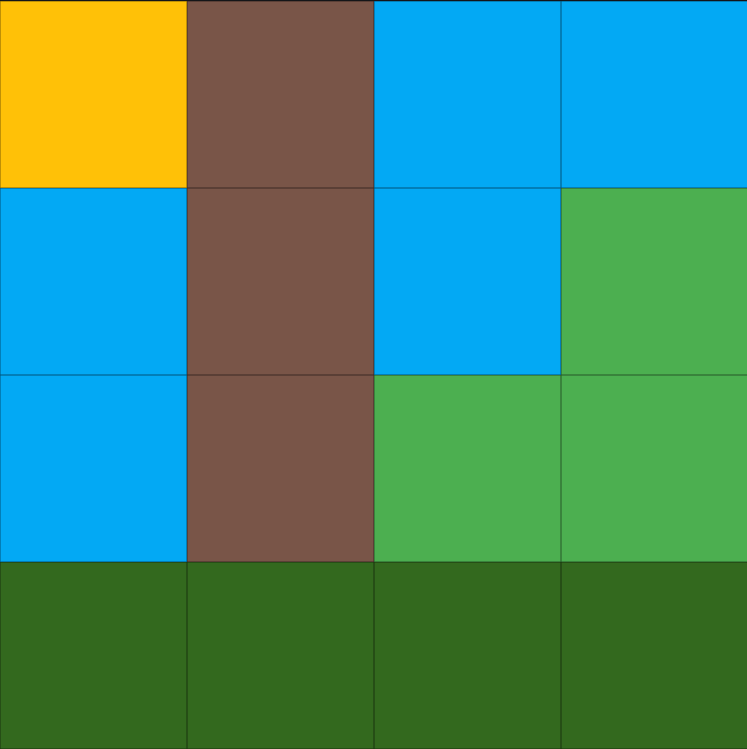
\includegraphics[width=\linewidth]{figures/image.png}
  \caption{Input Image}\label{fig:pixel_grid}
\endminipage\hspace{1em}
\minipage{0.40\textwidth}
  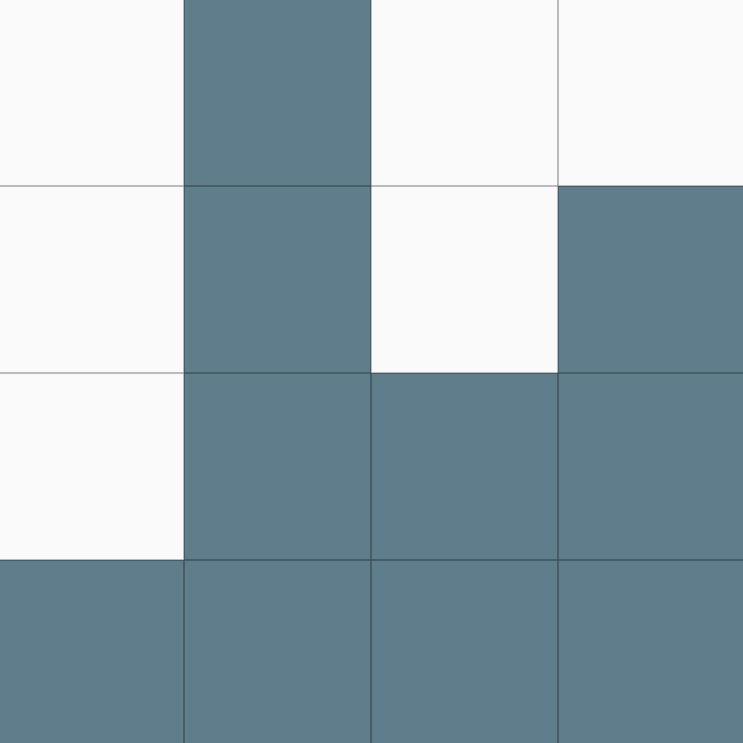
\includegraphics[width=\linewidth]{figures/class.png}
  \caption{Image Segmentation}\label{fig:seg_grid}
\endminipage
\end{figure}

Let's assume we have a 4 x 4 grid consisting of RGB pixels. Our task is to perform image segmentation, ie assign a label to each pixel from the set $\{\text{foreground}, \text{background}\}$. Intuitively, neighboring pixels should have similar values in y, i.e. pixels associated with a mountain should form one continuous blob. This knowledge can be naturally modeled via a Potts model which consists of potentials $\phi(y_i,x)$ that encode the likelihood that any given pixel is from our subject and  pairwise potentials $\phi(y_i,y_j)$ which will encourage adjacent 
y’s to have the same value with high probability. If visualized as a graphical model, we would have a node for each pixel and an edge for each pair of pixels that are touching vertically or horizontally but not diagonally. We will refer to these sets as $V$ and $E$ respectively.  
\newline
As seen in class, solving this task corresponds to finding $y$ such that

$$\hat{y} = \text{argmax}_{\boldsymbol{y}} \log_w p(y |x) $$
 $$=\text{argmax}_{\boldsymbol{y}}
 \sum_{j} w^T \phi(x_j, y_j) +
  \sum_{j,k \in E} w^T \phi(y_j, y_k)
 $$

\textcolor{red}{NOTE: This is not the same model used in the programming section. We will provide the set-up for that separately.}

\subsection{MAP Inference with Integer Linear Programming}

In this section, we will formulate our problem as an Integer Linear Program (ILP) and use it to predict the segmentation of a small patch of our image. For convenience, denote the background class with $0$ and the foreground class with $1$. Furthermore suppose we have variables $\alpha$ and $\beta$ that we will be optimizating over.  Let $\alpha_i(y)$ represent an indictator function that is one when pixel $i$ is labeled class $y$. Let $\beta_{ij}(y_n, y_m)$ represent an indicator function that is one when pixel $i$ is set to class $y_n$ and pixel $j$ is set to class $y_m$. 




First we will need to translate our requirements into a constraint set. 
\begin{questions}
\question[2] \textbf{Short answer:} Write constraints on the variables $\alpha_i(y)$ such that each pixel $i$ is assigned one and only one class $y$.

\begin{tcolorbox}[fit,height=2cm, width=15cm, blank, borderline={1pt}{-2pt}]
    % STUDENT SOLUTION HERE
    \end{tcolorbox}
    

\question[4] \textbf{Short answer:} Write constraints on the variables $\beta_{ij}(y_n, y_m)$ such that pixels $i$ and $j$ are consistently applied to the same classes $y_n$ and $y_m$ in the pairwise potentials. Note that this will only be defined over $ij$ pairs in our edge set $E$. 

\begin{tcolorbox}[fit,height=6cm, width=15cm, blank, borderline={1pt}{-2pt}]
    % STUDENT SOLUTION HERE
    \end{tcolorbox}



\question[2] \textbf{Short answer:} Using the score functions and goal defined above, write an ILP that represents our constraint set and objective such that if solved we would have a solution to our image segmentation task.

\begin{tcolorbox}[fit,height=8cm, width=15cm, blank, borderline={1pt}{-2pt}]
    % STUDENT SOLUTION HERE
    \end{tcolorbox}

\clearpage
Suppose we had the following unary feature functions:

\begin{equation*}
    \begin{split}
        \phi_1(\text{yellow pixel}, \text{background}) &= 1 \\
        \phi_2(\text{yellow pixel}, \text{foreground}) &= 2 \\
        \phi_3(\text{brown pixel}, \text{foreground}) &= 3 \\
        \phi_4(\text{brown pixel}, \text{background}) &= 0 \\
    \end{split}
\end{equation*}

In addition suppose we had the following non-zero pairwise feature functions:

\begin{equation*}
    \begin{split}
        \phi_5(\text{background}, \text{background}) &= 1 \\
        \phi_6(\text{foreground}, \text{background}) &= 2 \\
        \phi_7(\text{background}, \text{foreground}) &= 0 \\
        \phi_8(\text{foreground}, \text{foreground}) &= 1 \\
    \end{split}
\end{equation*}

\begin{figure}[!htb]
\centering
\minipage{0.25\textwidth}
  
\includegraphics[width=\linewidth]{figures/patch.png}
  \caption*{Image Patch}\label{fig:patch}
\endminipage\hspace{1em}
\minipage{0.25\textwidth}
  
\includegraphics[width=\linewidth]{figures/patch_labels.png}
  \caption*{Segmentation}\label{fig:patch_labels}
\endminipage
\caption{Extracted Image Patch and Segmentation}
\label{fig:path_q}
\end{figure}


\question[7]\label{q}\textbf{Short answer:}  In this question we will walk through the process of solving the ILP for the $1 \times 2$ patch in the upper left hand corner of our image shown in figure \ref{fig:path_q}. Assume an initial weight vector  $w = [1,1,1,...1]$.
\begin{parts}
    \part What are the scores assigned by the model for all possible y configurations shown below?
    \begin{center}
 \begin{tabular}{ |c|p{4cm}|p{4cm}|} 
 \hline
 \textbf{ } & \textbf{Yellow Background} & \textbf{Yellow Foreground}\\
 \hline
\textbf{Brown Background} &  & \\ 
 \hline
 \textbf{Brown Foreground}  &  &\\ 
 \hline
 
\end{tabular}
\end{center}

    
    \part What are the settings of variable $\alpha$ that solves the above ILP?
    \begin{tcolorbox}[fit,height=2cm, width=15cm, blank, borderline={1pt}{-2pt}]
    % STUDENT SOLUTION HERE
    \end{tcolorbox}
    
    \part What would be the updated weight vector $w$ after running one iteration of structured perceptron?
\begin{tcolorbox}[fit,height=2cm, width=15cm, blank, borderline={1pt}{-2pt}]
    % STUDENT SOLUTION HERE
    \end{tcolorbox}
    
\end{parts}





    
\question[5] \textbf{Short answer:} Assume the same set-up as seen in question \ref{q}. Also assume an initial weight vector  $w = [1,1,1,...1]$ and the Hamming loss as $l$. 


\begin{parts}
    \part What are the loss augmented scores for all possible y configurations shown below?
    \begin{center}
 \begin{tabular}{ |c|p{4cm}|p{4cm}|} 
 \hline
 \textbf{ } & \textbf{Yellow Background} & \textbf{Yellow Foreground}\\
 \hline
\textbf{Brown Background} &  & \\ 
 \hline
 \textbf{Brown Foreground}  &  &\\ 
 \hline
 
\end{tabular}
\end{center}




    
\part What would be the updated weight vector $w$ after running one iteration of structured SVM?
\begin{tcolorbox}[fit,height=2cm, width=15cm, blank, borderline={1pt}{-2pt}]
    % STUDENT SOLUTION HERE
    \end{tcolorbox}
    \end{parts}



\clearpage
\end{questions}
\begin{questions}
\fullwidth{\subsection{Loss-Augmented Inference and Learning}}

\question[1] \textbf{Select all that apply:} Structured Perceptron differs from Structured SVM in?
    {%
    \checkboxchar{$\Box$} \checkedchar{$\blacksquare$} % change checkbox style locally
    \begin{checkboxes}
     \choice Training
     \choice Inference
     \choice Evaluation
    \end{checkboxes}
    }
    
\question[4] 
Suppose you are given an MRF's factor graph $\Gc = (\Cc, \psi, \yv)$ consisting of a set of factors $\Cc$, potential functions $\psi$, and variables $\yv \in \Yc$, where $\Yc$ is the output space. Each factor $c \in \Cc$ touches a subset of the variables $\yv_c = [y_{c_1}, y_{c_2}, \ldots, y_{c_m}]^T$. The probability distribution defined by this graph decomposes multiplicatively according to the factors:
\begin{align*}
    p_{\Gc}(\yv) = \frac{1}{Z} \prod_{c \in \Cc} \psi_c(\yv_c)
\end{align*}
Further, you are given a loss function that decomposes additively according to the factors:
\begin{align*}
    \ell(\yv^*, \hat{\yv}) = \sum_{c \in \Cc} \ell_c(\yv_c^*, \hat{\yv}_c)
\end{align*}
% Finally, suppose that you have an algorithm that computes the most probable assignment $\yv^{(MAP)}$ to the variables in polynomial time:
% \begin{align*}
%     \yv^{(MAP)} \triangleq \argmax_{\yv \in \Yc} p(\yv)
% \end{align*}
Show that you can define a new factor graph $\Gc'$ (with the same factors and variables as $\Gc$, but different potential functions $\psi'$) such that the most probable assignment to $\hat{\yv}' \triangleq \argmax_{\yv \in \Yc} p_{\Gc'}(\yv)$ solves the loss-augmented MAP inference problem for $\Gc$ with loss $\ell$.
    \begin{tcolorbox}[fit,height=12cm, width=15cm, blank, borderline={1pt}{-2pt}]
    % STUDENT SOLUTION HERE
    \end{tcolorbox}
    
\end{questions}

\clearpage
\subsection{Empirical Questions}

The following questions should be completed after you work through the programming portion of this assignment (Section \ref{sec:code}). 

\begin{questions}
\question[12] Report the mean IOU and pixel accuracy scores for all models. For this question, you should run the FCN for 2 epochs and the linear SVM and structured SVM for 3 epochs each. \emph{Round each value to two significant figures}
\bgroup
\def\arraystretch{1.5}
\begin{center}
\begin{tabular}{ |c|p{2cm}|p{3cm}| } 
 \hline
 \textbf{Model} & \textbf{Mean IOU} &  \textbf{Pixel Accuracy} \\
 \hline
FCN (Train) &  & \\ \hline
FCN (Test) &  &  \\ \hline
FCN+l-SVM (Train) &  &  \\ \hline
FCN+l-SVM (Test) &  &  \\ \hline
FCN+s-SVM (Train) &  &  \\ \hline
FCN+s-SVM (Test) &  &  \\ \hline
\end{tabular}
\end{center}
\egroup

\question[10] Plot training and testing curves for the hinge loss (FCN+l-SVM) and structured hinge loss (FCN+s-SVM) respectively over 3 epochs. \emph{Note: Your plot must be machine generated.}
\begin{tcolorbox}[fit,height=12cm, width=15cm, blank, borderline={1pt}{-2pt}]
% STUDENT SOLUTION HERE
\end{tcolorbox}

\question[3] For any image of your choice from the test set, plot the labels predicted by FCN, FCN+l-SVM and FCN+s-SVM as grayscale images. Use the visualization function provided in the code to plot images. Do you see any remarkable differences between the model predictions?
\begin{tcolorbox}[fit,height=12cm, width=15cm, blank, borderline={1pt}{-2pt}]
% STUDENT SOLUTION HERE
\end{tcolorbox}

\end{questions}

\subsection{Wrap-up Questions}

\begin{questions}

\question[1] \textbf{Multiple Choice:} Did you correctly submit your code to Autolab?
    \begin{checkboxes}
     \choice Yes 
     \choice No
    \end{checkboxes}

\question[1] \textbf{Numerical answer:} How many hours did you spend on this assignment?.
    \begin{tcolorbox}[fit,height=1cm, width=2cm, blank, borderline={1pt}{-2pt}]
    % STUDENT SOLUTION HERE
    \end{tcolorbox}

\end{questions}

\clearpage
\subsection{Collaboration Policy}

    After you have completed all other components of this assignment, report your answers to the collaboration policy questions detailed in the Academic Integrity Policies for this course.
    \begin{enumerate}
        \item Did you receive any help whatsoever from anyone in solving this assignment? If so, include full details including names of people who helped you and the exact nature of help you received.
        
        \begin{tcolorbox}[fit,height=4cm, width=15cm, blank, borderline={1pt}{-2pt},nobeforeafter]
        % Place your solution between the comment lines below.
        % Do not modify the tcolorbox.
        % ----------------------------------------------------
        % STUDENT SOLUTION HERE
        % ----------------------------------------------------
       \end{tcolorbox}
        \item Did you give any help whatsoever to anyone in solving this assignment? If so, include full details including names of people you helped and the exact nature of help you offered.
        
        \begin{tcolorbox}[fit,height=4cm, width=15cm, blank, borderline={1pt}{-2pt},nobeforeafter]
        % Place your solution between the comment lines below.
        % Do not modify the tcolorbox.
        % ----------------------------------------------------
        % STUDENT SOLUTION HERE
        % ----------------------------------------------------
       \end{tcolorbox}
        \item Did you find or come across code that implements any part of this assignment? If so, include full details including the source of the code and how you used it in the assignment.
        
        \begin{tcolorbox}[fit,height=4cm, width=15cm, blank, borderline={1pt}{-2pt},nobeforeafter]
        % Place your solution between the comment lines below.
        % Do not modify the tcolorbox.
        % ----------------------------------------------------
        % STUDENT SOLUTION HERE
        % ----------------------------------------------------
       \end{tcolorbox}
    \end{enumerate}
\clearpage
\section{Programming \pts{48} }
\label{sec:code}

Your goal in this assignment is to implement a structured SVM on top of a convolutional neural network for image segmentation. Given an image as a 32x32 grid of pixels, you will assign a label from the set $\{foreground, background\}$ to each pixel.


Your solution for this section must be implemented with \textbf{PyTorch} and \textbf{Google OR-Tools}\footnote{\url{https://developers.google.com/optimization}} using the data files we have provided to you. This restriction is because we will be grading your code by hand to check your understanding as well as your model's performance. 

\subsection{Task Background}
Semantic segmentation is the task of assigning a class label to each pixel in an image. This task can be thought of as image classification, but at the pixel level. Figure \ref{fig:seg_example} shows a sample image with its corresponding segmented image.
\begin{figure}[h]
\centering
\begin{subfigure}{.5\textwidth}
  \centering
  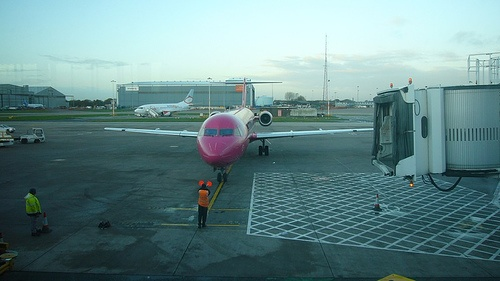
\includegraphics[width=.7\linewidth]{figures/orig_image.jpg}
  \caption{Original Image}
\end{subfigure}%
\begin{subfigure}{.5\textwidth}
  \centering
  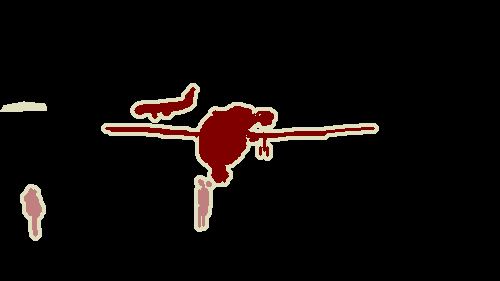
\includegraphics[width=.7\linewidth]{figures/seg_image.png}
  \caption{Segmented Image}
\end{subfigure}
\caption{Sample image from the PASCAL VOC-2012 Image Segmentation dataset}
\label{fig:seg_example}
\end{figure}

Semantic segmentation is useful for a variety of applications such as autonomous vehicles, photo-editing tools and many tasks in robotics. In this question, we will first train a simple semantic segmentation model using a fully convolutional network (FCN). Next, we will use this FCN as a feature extractor to generate 100-dimensional features for each pixel in the image. Using these pixel features, we will build two semantic segmentation models. The first baseline model is a simple linear support vector machine (SVM) which uses the FCN features and predicts a class label for each pixel in the image independently. The second model is a structured SVM which takes in FCN features and predicts class labels for all pixels in the image while incorporating interactions between neighboring pixels. Following subsections provide more details about the dataset, metrics and model structure.

\subsection{Data}
For this task, we will be using the semantic segmentation dataset from the PASCAL VOC 2012 Challenge.\footnote{\url{http://host.robots.ox.ac.uk/pascal/VOC/voc2012/index.html}} This dataset consists of 2913 examples in total (2330 for training and 583 for testing). For each example in this dataset, we have a pair of images: the original image and the segmented image. To make it easier to work with the data, we have converted segmented images into numpy arrays of class labels. To ensure reasonable runtime, we have also cropped and downsampled all images to 32x32 pixels. Finally, instead of having multiple class labels (eg: person, aeroplane etc.), we will treat this as a binary classification task with the label set $\{foreground, background\}$.

\subsection{Metrics}
To evaluate model performance on this dataset, we will be using two metrics:
\begin{itemize}
    \item \textbf{Pixel Accuracy:} Pixel-level classification accuracy for each image computed as\\
    \begin{align}
    \frac{\#CorrectPixels}{\#TotalPixels}
    \end{align}
    \item \textbf{Mean IOU (Intersection-over-Union):} Mean of per-class IOU (intersection-over-union) across all classes for each image. For one class (eg: foreground), IOU is computed as \\
    \begin{align}
        \frac{\#CorrectForegroundPixels}{\#GoldForegroundPixels + \#PredictedForegroundPixels - \#CorrectForegroundPixels}
    \end{align}
\end{itemize}{}
We will average these metrics across all images

\subsection{Fully Convolutional Network}
As a first step towards building a semantic segmentation model, we will train a fully convolutional network. A fully convolutional network differs from a regular convolutional neural network in the later half of its architecture. While a convolutional neural network returns a dense representation for each image (eg: a 6x6 representation for a 32x32 image), a fully convolutional network returns a representation of the same size as the original image. FCNs use regular convolution layers to first compress an image into a dense representation before \emph{deconvolving} the dense representation to get a tensor of the same size as the original image (as shown in figure \ref{fig:fcn}). 

\begin{figure}[h]
    \centering
    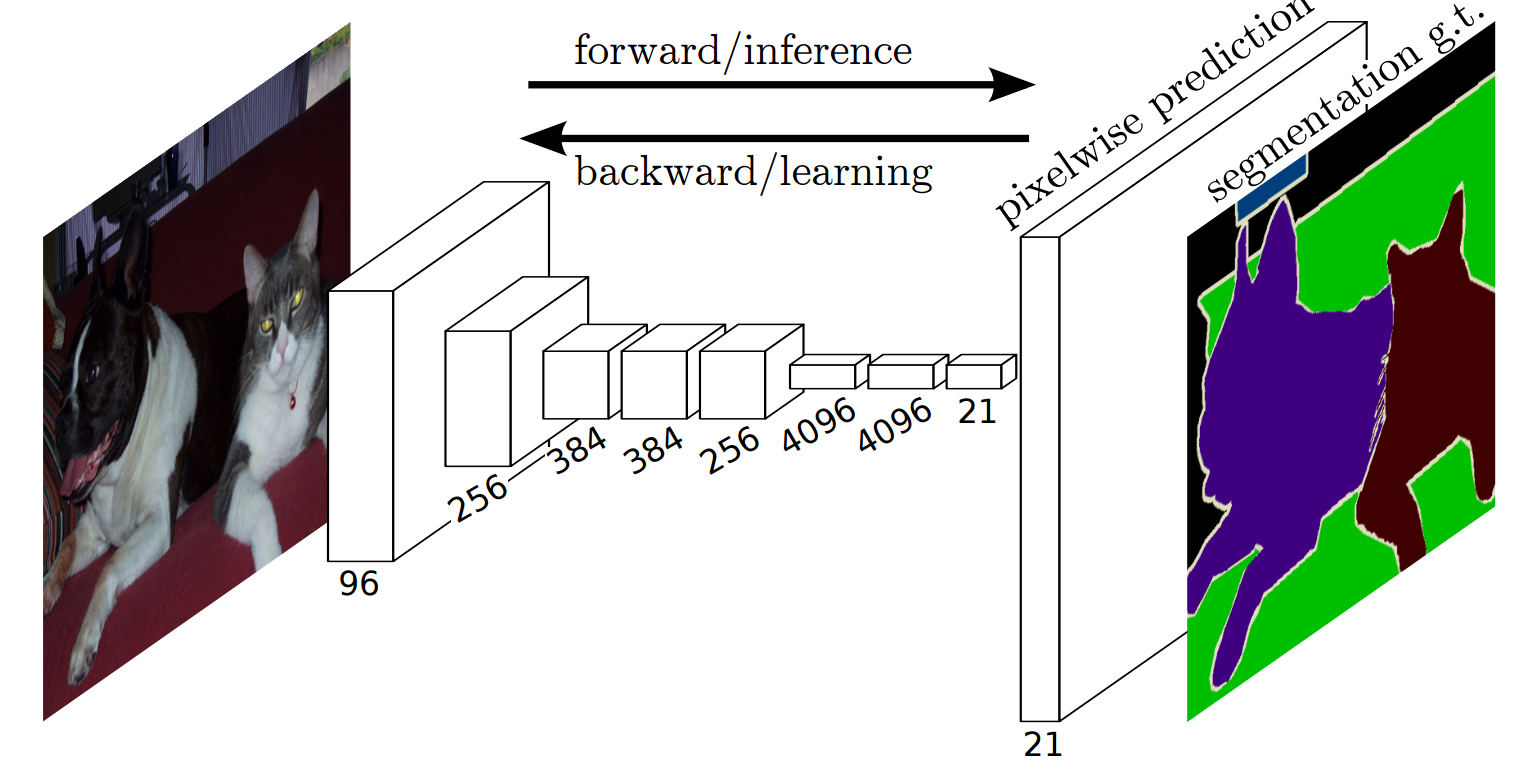
\includegraphics[scale=0.2]{figures/fcn_segmentation.png}
    \caption{Fully convolutional network for semantic segmentation}
    \label{fig:fcn}
\end{figure}

For this assignment, we have provided you with code to train and test a FCN. Our FCN implementation uses the first 5 layers from AlexNet as convolution layers and an interpolation layer to perform the deconvolution. After running the FCN on a 32x32 image, you should be able to extract a 32x32x100 tensor which contains a 100-dimensional feature vector for each pixel. We add an additional 100x2 linear layer to predict (foreground, background) scores for each pixel and train this network using cross-entropy loss. After training, we discard the linear layer and use the FCN weights to generate pixel-level features for a given image.

\subsection{Baseline}
The first model you will be implementing is a simple linear support vector machine. This model takes as input a 32x32x100 tensor computed by the FCN and uses weights $w_{fc}$ to calculate per-class scores for each pixel independently. This is analogous to simply adding a linear layer on top of the FCN. However, since the baseline is a linear SVM, it is trained using hinge loss. (\textbf{Hint:} To implement hinge loss in PyTorch, you might find it helpful to look up MultiMarginLoss()). 

\subsection{Main Model}
The second model you will be implementing is a structured support vector machine. Unlike the linear SVM, this model does not predict labels for each pixel independently. This is useful because adjacent pixels tend to belong to the same class, indicating that there may be some benefits to treating this problem as a structured prediction problem and leveraging pixel interactions. In this assignment, we will model the structure of the output using a formulation based on associative markov networks.\footnote{\url{https://ai.stanford.edu/~koller/Papers/Taskar+al:ICML04.pdf}} Associative markov networks are a class of undirected graphical models where each node is a discrete variable and clique potentials tend to favor the same label for all nodes in the clique. 
In our task, we treat each pixel as a node and only model pairwise interactions between pixels (i.e no cliques larger than 2 exist). For tractability, we further restrict pairwise interactions to non-diagonal neighboring pixels (up, down, left, right). This results in a lattice structure as shown in the figure:
\begin{figure}[h]
    \centering
    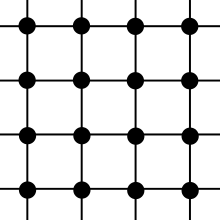
\includegraphics[scale=0.5]{figures/lattice.png}
    \caption{Output structure used by structured SVM}
    \label{fig:lattice}
\end{figure}

Given an input image as a 32x32x100 feature tensor $T$ extracted from the FCN, a SVM over this structured output space can be formulated as follows:
\noindent
\begin{itemize}
    \item \textbf{Variables:} $x_{i,c}$ where $i \in [0,32*32), c \in \{0,1\}$, $y_{i,j,c}$, where $i \in [0,32*32), j \in [0,32*32), c \in \{0,1\}$. $x_{i,c}$ and $y_{i,j,c}$ are pixel assignment and edge assignment variables respectively. $x_{i,c} = 1$ indicates that pixel at position $i$ belongs to class $c$, while $y_{i,j,c} = 1$ indicates that pixels in neighboring positions $i$ and $j$ both belong to class $c$ and are linked to one another.
    \item \textbf{Weights:} $w_{f,c}$ and $w_{f',c}$, where $f \in [0,100), f' \in [0,200), c \in \{0,1\}$. $w_{f,c}$ and $w_{f',c}$ are pixel weights and edge weights respectively. These weights can be used to compute unary pixel potentials and edge potentials as $\phi_{i,c} = w_{f,c} T(i)$ and $\phi_{i,j,c} = w_{f',c} concat(T(i), T(j))$. Recall that we used a similar process in homework 2 to compute unary/ edge potentials for nodes in the parse tree from LSTM hidden states.
    \item \textbf{ILP formulation for MAP inference:} Using the pixel and edge potentials computed using weights and FCN features, the highest scoring output structure (i.e. the assignment of values to $x_{i,c}, y_{i,j,c}$) is chosen by maximizing the following objective:\\
    \begin{align*}
     \max_{\xv, \yv} \sum_i \sum_c \phi_{i,c} x_{i,c} + \sum_i \sum_j \sum_c \phi_{i,j,c} y_{i,j,c} 
    \end{align*}
    subject to the following constraints:\\
    \begin{align*}
        \sum_c x_{i,c} &= 1\\
        y_{i,j,c} &\leq x_{i,c}\\
        y_{i,j,c} &\leq x_{j,c}
    \end{align*}
    The first constraint ensures that each pixel is assigned to exactly one class, while the next two constraints ensure that if an edge exists between two pixels, they both belong to the same class.

\item 
    \recentChange{
    \textbf{Loss-augmented Inference:} To define loss-augmented inference, we need a loss function. We choose $\ell(\hat \xv, \xv^*)$ to be the Hamming loss between the two outputs:
    \begin{align*}
        \ell(\hat \xv, \xv^*) = \frac{1}{|i||c|} \sum_i \sum_c \ind{\hat{x}_{i,c} \neq x^*_{i,c}}
    \end{align*}
    Setting up an ILP for loss-augmented inference uses the exact same constraints as the MAP Inference ILP above, but we change the objective function to be the following:
    \begin{align*}
     \max_{\xv, \yv}  \sum_i \sum_c \phi_{i,c} x_{i,c} + \sum_i \sum_j \sum_c \phi_{i,j,c} y_{i,j,c} 
       + \frac{1}{|i||c|} \sum_i \sum_c \left( x^*_{i,c} (1 - x_{i,c}) + (1 - x^*_{i,c}) x_{i,c} \right)
    \end{align*}
    
    
\item \textbf{Loss function:} The structured hinge loss for this SVM is as follows:\\
    \begin{align*}
        L = \max(0, S(\hat \xv, \hat \yv,  T) + \ell(\hat \xv, \xv^*) - S(\xv^*, \yv^*, T))
    \end{align*}
    where the scoring function $S(\xv, \yv, T) = \sum_i \sum_c \phi_{i,c} x_{i,c} + \sum_i \sum_j \sum_c \phi_{i,j,c} y_{i,j,c}$ is the same as the ILP objective (note that the potentials $\phi$ in the objective are computed using vectors from $T$), and $(\hat{\xv}, \hat{\yv})$ is the highest scoring structure returned by loss-augmented inference, and $(\xv^*, \yv^*)$ is the ground truth assignment to pixel/edge variables.
    
    }
\end{itemize}

Putting everything together, given an image $I$, you should run the following procedure:
\begin{enumerate}
    \item Extract feature tensor $T = FCN(I)$
    \item Compute pixel and edge potentials $\phi_{i,c}, \phi_{i,j,c}$ using $T$
    \item Perform \recentChange{loss-augmented MAP inference} via ILP to get highest scoring structure $(\hat\xv, \hat\yv)$
    \item Compute structured hinge loss with $(\hat\xv, \hat\yv)$
    \item Backpropagate through the structured loss to update weights
\end{enumerate}
At test time, \recentChange{you only need to return the most probable assignment as your output (i.e. step 3 below does not augment with the loss). 
\begin{enumerate}
    \item Extract feature tensor $T = FCN(I)$
    \item Compute pixel and edge potentials $\phi_{i,c}, \phi_{i,j,c}$ using $T$
    \item Perform MAP inference via ILP to get highest scoring structure $(\hat\xv,\hat\yv)$
\end{enumerate}
}
\subsection{Implementation Details}
We have provided you with some starter code (starter\_code.py). You should be able to simply run this starter code to train and test a FCN on the data after adding the correct paths. You are expected to implement both SVM models by filling in the TODOs. The reference SVM implementation uses Adam optimizer with learning rate 0.0001 for both linear and structured SVM. It also uses class weights for the linear model (similar to the FCN) to handle the class imbalance issue. You should train the FCN in isolation for 2 epochs before using it as a feature extractor for any of the SVM models. Both SVM models only update their own weights and DO NOT update the FCN weights. Train both SVM models for 3 epochs each before answering the empirical questions. For ILP optimization, use the GLOP linear solver from OR-Tools. Though this solver optimizes the LP-relaxation instead of the ILP, the associative markov networks paper demonstrates that for our objective and constraints, the LP-relaxation and ILP have the same solution. (However, if the number of classes is greater than 2, this result does not hold!)

\subsection{Autolab Submission \pts{35}}

You must submit a .tar file named \lstinline{structuredsvm.tar} containing \lstinline{structuredsvm.py}, which contains all of your code.

You can create that file by running:
\begin{lstlisting}
tar -cvf structuredsvm.tar structuredsvm.py
\end{lstlisting}
from the directory containing your code.

Some additional tips: {\bf DO NOT} compress your files; you are just
creating a tarball. Do not use tar \texttt{-czvf}.  {\bf DO NOT} put
the above files in a folder and then tar the folder.  Autolab is case
sensitive, so observe that all your files should be named in {\bf
  lowercase}. You must submit this file to the corresponding homework
link on Autolab. 

Your code will \textbf{not} be autograded on Autolab. Instead, we will grade your code by hand; that is, we will read through your code in order to grade it. As such, please carefully identify major sections of the code via comments. 




\end{document}
